\documentclass[../report.tex]{subfiles}

\begin{document}

\graphicspath{{img/}{../img/}}

\section{SCRUM men... Ikke helt}


\paragraph{Hvad er scrum?}
Scrum er en agil software udviklings metode, hvis hovedm�l er at kunne h�ndtere �ndringer i kravspecifikationen mens udviklingen er i gang. Indenfor godtagelse af krav�ndringer er scrum mods�tningen til vandfaldsmodellen, som ikke tager sig p�nt i et milj� med mange krav �ndringer.

\paragraph{scrum men... Hvad mangler s�?} I target-projektet bliver der arbejdet efter scrum ? men ikke scrum i dets fulde forstand. I det projekt har blev det besluttet at k�re l�st p� nogle af scrums discipliner, fordi der var enighed om at det ikke gav meget mening for en projekt gruppe der kun m�des et par gange om ugen.\\


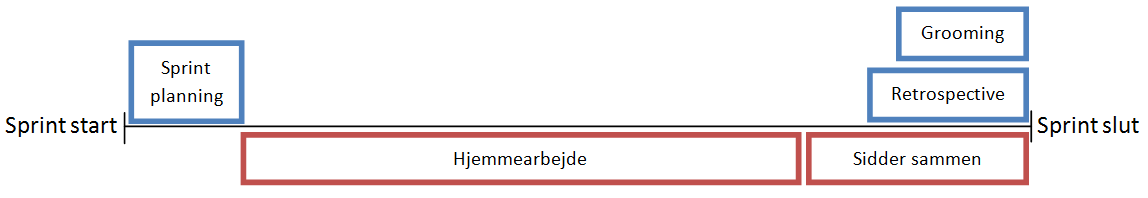
\includegraphics[scale=0.8]{SCRUMtimeLine.png}\\

\begin{tabularx}{14cm}{c|X}
\textbf{Aktiviteter}  & \textbf{�ndringer} \\
SCRUM roller & I et eksamensprojekt er det urealistisk at have en person til kun at v�re product owner. I target-projektet er product owner ene og alene ansvarlig for kommunikation med stakeholders og prioritering af product items, men han er ogs� udvikler i scrum teamet     \\ 
 & \\
Scrum Board & scrum boardet er den centrale oversigt over hvad der skal laves og er lavet. Boardet fungerer efter vores erfaringer ogs� som stor motivationsfaktor. Da projektgruppen i target-projektet ikke har et fast lokale, er et fysisk board dog ikke muligt, s� online v�rkt�jet Trello bliver brugt i stedet\footnote{Trello.com} \\
 & \\
Standup meeting & Da der i target-projektet ofte bliver arbejdet selvst�ndigt \\
 & \\
 & \\
 & \\
\end{tabularx} 


\end{document}